%====================================================
% Title Page definition
\thispagestyle{empty}
\begin{titlepage}
  \begin{center}
    \baselineskip=100pt
    {\fontsize{100}{120}\selectfont  \TT{Teoria Sygnałów}{Signal Theory}} \\[1em] {\fontsize{80}{100}\selectfont \TT{w zadaniach}{in practise}}
    \baselineskip=10pt
    \begin{minipage}[t]{0.4\textwidth}
    \vspace{2em}
    \begin{figure}[H]
      \centering
      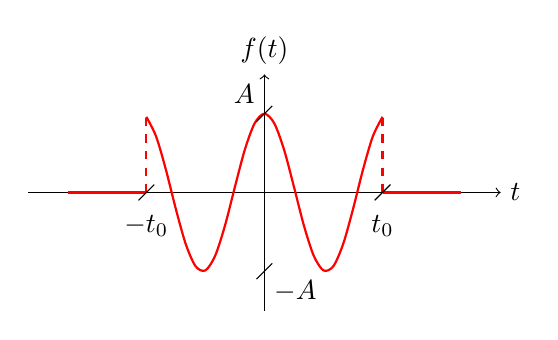
\begin{tikzpicture}
      %\draw (0,0) circle (1in);
      \draw[->] (-3.0,+0.0) -- (+3.0,+0.0) node[right] {$t$};
      \draw[->] (+0.0,-1.5) -- (+0.0,+1.5) node[above] {$f(t)$};
      \draw[-,red, thick] (-2.5,+0.0) -- (-1.5,0.0);
      \draw[-,red, thick] (+1.5,+0.0) -- (+2.5,0.0);
      \draw[scale=1.0,domain=-1.5:1.5,smooth,variable=\x,red,thick] plot ({\x},{1.0*cos(\x*180/3.141592*4.0)});%96%3.141592
      \draw[-,red, thick, dashed] (+1.5,+0.0) -- (+1.5,1.0);
      \draw[-,red, thick, dashed] (-1.5,+0.0) -- (-1.5,1.0);
      
      
      \draw[-] (-1.5-0.1,-0.1)--(-1.5+0.1,0.1) node[midway, below, outer sep=5pt,align=center] {$-t_0$};
      \draw[-] (+1.5-0.1,-0.1)--(+1.5+0.1,0.1) node[midway, below, outer sep=5pt] {$t_0$};
      \draw[-] (-0.1,+1.0-0.1)--(+0.1,+1.0+0.1) node[midway, above left] {$A$};
      \draw[-] (-0.1,-1.0-0.1)--(+0.1,-1.0+0.1) node[midway, below right] {$-A$};
      \end{tikzpicture}
    \end{figure}
    \begin{equation*}
    f(t)=A\cdot \Pi\left(\frac{t}{2\cdot t_0}\right)\cdot cos\left(\frac{2\pi}{t_0}\cdot t\right)
    \end{equation*}
    \end{minipage}
    \begin{minipage}[t]{0.4\textwidth}
    \begin{figure}[H]
      \centering
      \begin{tikzpicture}
      \draw[->] (-3.0,+0.0) -- (+3.0,+0.0) node[right] {$\omega$};
      \draw[->] (+0.0,-0.5) -- (+0.0,+3.0) node[above] {$\left|F(\jmath \cdot \omega)\right|$};
      
      \draw[scale=1.0,domain=-2.5:2.5,samples=2000,smooth,variable=\x,red,thick] plot ({\x},{abs(-2*sinc((\x-1.0)*3.141592*4)+2*sinc((\x+1.0)*3.141592*4))});
      
      \draw[-] (-1.0-0.1,-0.1)--(-1.0+0.1,0.1) node[midway, below, outer sep=5pt] {-$\frac{2\pi}{t_0}$};
      \draw[-] (+1.0-0.1,-0.1)--(+1.0+0.1,0.1) node[midway, below, outer sep=5pt] {$\frac{2\pi}{t_0}$};
      \draw[-] (-0.1,+2.0-0.1)--(+0.1,+2.0+0.1) node[midway, above right] {$A \cdot t_0$};
      %\draw[-] (-0.1,-2.0-0.1)--(+0.1,-2.0+0.1) node[midway, below right] {$-A\cdot t_0$};      
      \end{tikzpicture}
    \end{figure}
    \begin{align*}
    F(\jmath \omega)=A \cdot t_0 \cdot \left[ \right.&\left. Sa\left(\omega \cdot t_0 + 2\pi\right) \right.\\
    &\left.- Sa\left(\omega \cdot t_0 - 2\pi\right)\right]
    \end{align*}
    \end{minipage}    
    \\[6em]
    \bookauthors
    
    \vfill
    
    % Bottom of the page
    %{\large \date }
    {\large \today }
    
  \end{center}
\end{titlepage}
\cleardoublepage
%====================================================